\documentclass{beamer}
\setbeamertemplate{footline}[frame number]

\ifx\pdfoutput\undefined
%  \usepackage{graphicx}
\else
%  \usepackage[pdftex]{graphicx}
  \DeclareGraphicsRule{*}{mps}{*}{}
\fi

%%\documentclass[landscape]{slides}
%\AtBeginDocument{%
%  \pdfpageheight = \paperheight
%  \pdfpagewidth = \paperwidth
%}

%%\usepackage{times}
\usepackage{color}
\usepackage{latexsym}
%\usepackage{graphicx}

\raggedright

\definecolor{bgblue}{rgb}{0.04,0.39,0.53}

%\newcommand{\argmax}[1]{\begin{array}{c}\mbox{arg max}\\#1\end{array}}

\begin{document}


\title{\color{blue}Natural Language Processing}

\author{Anoop Sarkar \\ {\tt http://anoopsarkar.github.io/nlp-class}}
\institute{}
%\date{}
     
{
\setbeamertemplate{navigation symbols}{}
\addtocounter{framenumber}{-1}
\begin{frame}
\begin{center}
\vspace{1cm}
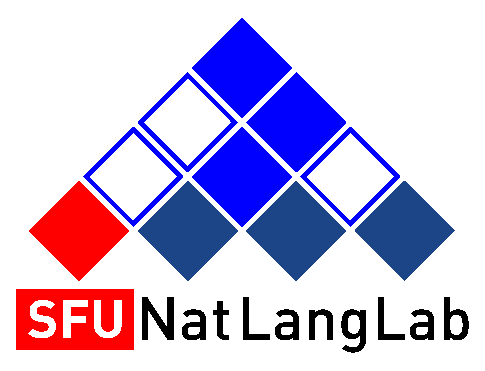
\includegraphics[scale=0.4]{figures/natlang-cky-logo.eps}
\end{center}
\titlepage
\end{frame}
}



\section{Smoothing $n$-gram Models}
\frame{\tableofcontents[currentsection]}

\subsection{Event Space for $n$-gram Models}

\begin{frame}
\frametitle{Trigram Models}
\begin{itemize}[<+->]
\item The trigram model:\\
$P(w_1, w_2, \ldots, w_n) = P(w_1) \times P(w_2~\mid~w_1) \times 
P(w_3~\mid~w_1, w_2) \times P(w_4~\mid~w_2, w_3) 
\times \ldots P(w_i~\mid~w_{i-2}, w_{i-1}) \ldots 
\times P(w_n~\mid~w_{n-2}, \ldots, w_{n-1}) $
\item Notice that the length of the sentence $n$ is variable
\item What is the event space?
\end{itemize}
\end{frame}

\newcommand{\lmstop}{\mbox{\texttt stop}}

\begin{frame}
\frametitle{The {\tt stop} symbol}
\begin{itemize}[<+->]
\item Let ${\cal V} = \{ a, b \}$ and the language $L$ be ${\cal V}^\ast$
\item Consider a unigram model: $P(a) = P(b) = 0.5$
\item So strings in this language $L$ are:
\begin{eqnarray*}
a\ \lmstop & 0.5 \\
b\ \lmstop & 0.5 \\
aa\ \lmstop & 0.5^2 \\
bb\ \lmstop & 0.5^2 \\
\vdots
\end{eqnarray*}
\item The sum over all strings in $L$ should be equal to 1:
\[ \sum_{w \in L} P(w) = 1 \]
\item But $P(a) + P(b) + P(aa) + P(bb) = 1.5$ !! 
\end{itemize}
\end{frame}


\begin{frame}
\frametitle{The {\tt stop} symbol}
\begin{itemize}[<+->]
\item What went wrong? \\
We need to model variable length sequences
\item Add an explicit probability for the \lmstop symbol: 
\[ P(a) = P(b) = 0.25  \]
\[ P(\lmstop) = 0.5 \]
\item $P(\lmstop) = 0.5$, $P(a\ \lmstop) = P(b\ \lmstop) = 0.25 \times 0.5 = 0.125$, 
$P(aa\ \lmstop) = 0.25^2 \times 0.5 = 0.03125$ (now the sum is no longer greater than one)
\end{itemize}
\end{frame}

\begin{frame}
\frametitle{The {\tt stop} symbol}
\begin{itemize}[<+->]
\item With this new {\tt stop} symbol we can show that $\sum_w P(w) = 1$ \\
Notice that the probability of any sequence of length $n$ is $0.25^n \times 0.5$ \\
Also there are $2^n$ sequences of length $n$
\end{itemize}
\begin{eqnarray}
\lefteqn{\sum_w P(w) = } \nonumber \\
&& \sum_{n=0}^{\infty} 2^n \times 0.25^n \times 0.5 \nonumber \\
&& \sum_{n=0}^{\infty} 0.5^n \times 0.5 = \sum_{n=0}^{\infty} 0.5^{n+1} \nonumber \\
&& \sum_{n=1}^{\infty} 0.5^n = 1 \nonumber
\end{eqnarray}
\end{frame}

\subsection{Smoothing Counts}

\begin{frame}
\frametitle{Bigram Models}
\begin{itemize}[<+->]
\item
In practice: 
\begin{eqnarray*}
\lefteqn{P(\textsf{Mork read a book})=}\\
&& P(\textsf{Mork}~\mid~<\textsf{start}>) \times P(\textsf{read}~\mid~\textsf{Mork}) \times \\
&& P(\textsf{a}~\mid~\textsf{read}) \times P(\textsf{book}~\mid~\textsf{a}) \times \\
&& P(<\textsf{stop}>~\mid~\textsf{book})
\end{eqnarray*}

\item $P(w_i~\mid~w_{i-1}) = \frac{ c(w_{i-1},w_i) } { c(w_{i-1}) }$ \\
 On unseen data, $c(w_{i-1},w_i)$ or worse $c(w_{i-1})$ could be zero
\[ \sum_{w_i} \frac{ c(w_{i-1},w_i) } { c(w_{i-1}) } = ? \]

\end{itemize}
\end{frame}


\begin{frame}
\frametitle{Smoothing}
\begin{itemize}[<+->]

\item {\bf Smoothing} deals with events that have been observed zero times

\item Smoothing algorithms also tend to improve the accuracy of the model

\[ P(w_i~\mid~w_{i-1}) = \frac{ c(w_{i-1},w_i) } { c(w_{i-1}) } \]

\item Not just unobserved events: what about events observed once?
\end{itemize}
\end{frame}

\subsubsection{Add-one Smoothing}

\begin{frame}
\frametitle{Add-one Smoothing}
\[ P(w_i~\mid~w_{i-1}) = \frac{ c(w_{i-1},w_i) } { c(w_{i-1}) } \]
\begin{itemize}[<+->]
\item Add-one Smoothing:
\[ P(w_i~\mid~w_{i-1}) = \frac{ 1 + c(w_{i-1},w_i) } { V + c(w_{i-1}) } \]
\item Let $V$ be the number of words in our vocabulary \\
 Assign count of $1$ to unseen bigrams
\end{itemize}
\end{frame}

\begin{frame}
\frametitle{Add-one Smoothing}
\begin{eqnarray*}
\lefteqn{P(\textsf{Mindy read a book})=}\\
&& P(\textsf{Mindy}~\mid~<\textsf{start}>) \times P(\textsf{read}~\mid~\textsf{Mindy}) \times \\
&& P(\textsf{a}~\mid~\textsf{read}) \times P(\textsf{book}~\mid~\textsf{a}) \times \\
&& P(<\textsf{stop}>~\mid~\textsf{book})
\end{eqnarray*}
\begin{itemize}[<+->]
\item Without smoothing:
\[ P(\textsf{read}~\mid~\textsf{Mindy}) = \frac{ c(\textsf{Mindy, read}) } { c(\textsf{Mindy}) }  = 0 \]
\item With add-one smoothing (assuming c(Mindy) = 1 but c(Mindy, read)
  = 0):
\[ P(\textsf{read}~\mid~\textsf{Mindy}) = \frac{ 1 } { V + 1 }  \]
\end{itemize}
\end{frame}

\subsubsection{Additive Smoothing}

\begin{frame}
\frametitle{Additive Smoothing: (Lidstone 1920, Jeffreys 1948)} 
\[ P(w_i~\mid~w_{i-1}) = \frac{ c(w_{i-1},w_i) } { c(w_{i-1}) } \]
\begin{itemize}[<+->]
\item Add-one smoothing works horribly in practice. Seems like $1$ is too large a count for unobserved events.
\item Additive Smoothing:
\[ P(w_i~\mid~w_{i-1}) = \frac{ \delta + c(w_{i-1},w_i) } { (\delta \times V) + c(w_{i-1}) } \]
\item $0 < \delta \leq 1$ \\
Still works horribly in practice, but better than add-one smoothing.
\end{itemize}
\end{frame}

\subsubsection{Good-Turing Smoothing}

\begin{frame}
\frametitle{Good-Turing Smoothing: (Good, 1953)} 
\[ P(w_i~\mid~w_{i-1}) = \frac{ c(w_{i-1},w_i) } { c(w_{i-1}) } \]
\begin{itemize}[<+->]
\item Imagine you're sitting at a sushi bar with a conveyor belt. 
\item You see going past you  { \color{blue} 10} plates of tuna,  { \color{blue} 3} plates of unagi,  { \color{blue} 2} plates of salmon,  { \color{blue} 1} plate of shrimp,  { \color{blue} 1} plate of octopus, and  { \color{blue} 1} plate of yellowtail
\item Chance you will observe a \alert{new} kind of seafood: {\color{blue} $\frac{3}{18}$}
\item How likely are you to see another plate of salmon: \\
should be { \color{blue} $< \frac{2}{18}$ }
\end{itemize}
\end{frame}

\begin{frame}
\frametitle{Good-Turing Smoothing}
\begin{itemize}[<+->]
\item How many types of seafood (words) were seen once? Use this to predict probabilities for unseen events\\
Let $n_1$ be the number of events that occurred once: 
{ \color{blue} $p_0 = \frac{ n_1 }{ N } $}
\item The Good-Turing estimate states that for any $n$-gram that occurs $r$ times, we should pretend that it occurs $r^\ast$ times
{\color{blue} \[ r^\ast = (r+1) \frac{ n_{r+1} }{ n_r } \] }
\item {\color{blue} $n_r$}: number of different objects seen $r$ times
\end{itemize}
\end{frame}

\begin{frame}
\frametitle{Good-Turing Smoothing}
\begin{itemize}[<+->]
\item { \color{blue} 10} tuna,  { \color{blue} 3} unagi,  { \color{blue} 2} salmon,  { \color{blue} 1} shrimp,  { \color{blue} 1} octopus,  { \color{blue} 1} yellowtail
\item How likely is new data? Let $n_1$ be the number of items occurring once, which is {\color{blue} 3} in this case. $N$ is the total, which is {\color{blue} 18}.
\[ p_0 = \frac{n_1}{N} = \frac{3}{18} = 0.166 \]
\end{itemize}
\end{frame}

\begin{frame}
\frametitle{Good-Turing Smoothing}
\begin{itemize}[<+->]
\item { \color{blue} 10} tuna,  { \color{blue} 3} unagi,  { \color{blue} 2} salmon,  { \color{blue} 1} shrimp,  { \color{blue} 1} octopus,  { \color{blue} 1} yellowtail
\item How likely is {\em octopus}? Since $c(\textit{octopus}) = 1$ The GT estimate is $1^\ast$. 
{\color{blue} \[ r^\ast = (r+1) \frac{ n_{r+1} }{ n_r } \] }
{\color{blue} \[ p_{GT} = \frac{ r^\ast }{ N } \] }
\item To compute $1^\ast$, we need $n_1 = 3$ and $n_2 = 1$
\[ 1^\ast = 2 \times \frac{1}{3} = \frac{2}{3} \]
\[ p_1 = \frac{1^\ast}{18} = 0.037 \]
\item What happens when $n_{r+1} = 0$? (smoothing before smoothing)
\end{itemize}
\end{frame}

\begin{frame}
\frametitle{Simple Good-Turing: linear interpolation for missing $n_{r+1}$}
\begin{columns}[l]
\column{.7\textwidth}
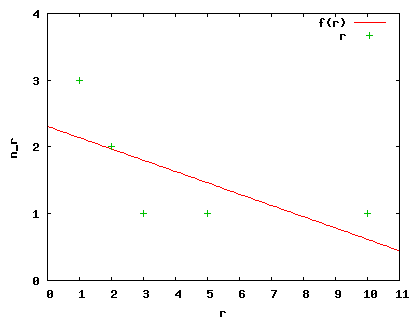
\includegraphics[scale=0.55]{figures/fit.png}
\column{.3\textwidth}
{\small
\begin{eqnarray*}
f(r) & = & a + b * r \\
a & = & 2.3 \\
b & = & -0.17 
\end{eqnarray*}
\begin{tabular}{ll}
\hline
$r$ & $n_r = f(r)$  \\
\hline
$1$ & 2.14 \\
$2$ & 1.97 \\
$3$ & 1.80 \\
$4$ & 1.63 \\
$5$ & 1.46 \\
$6$ & 1.29 \\
$7$ & 1.12 \\
$8$ & 0.95 \\
$9$ & 0.78 \\
$10$ & 0.61 \\
$11$ & 0.44 \\
\hline
\end{tabular}
}
\end{columns}
\end{frame}


\begin{frame}
\frametitle{Comparison between Add-one and Good-Turing}
\centering
\begin{tabular}{lllll}
\hline
freq & num with freq $r$ & NS    & Add1  & SGT   \\
$r$  & $n_r$ & $p_r$ & $p_r$ & $p_r$ \\
\hline
0  &  0 & 0    & 0.0294 & 0.12 \\
1  &  3 & 0.04 & 0.0588 & 0.03079 \\
2  &  2 & 0.08 & 0.0882 & 0.06719 \\
3  &  1 & 0.12 & 0.1176 & 0.1045 \\
5  &  1 & 0.2  & 0.1764 & 0.1797 \\
10 &  1 & 0.4  & 0.3235 & 0.3691 \\
\hline
\end{tabular}
\begin{itemize}[<+->]
\item $N = (1*3) + (2*2) + 3 + 5 + 10 = 25$
\item $V = 1 + 3 + 2 + 1 + 1 + 1 = 9$
\item Important: we added a new word type for unseen words. Let's call it UNK, the unknown word.
\item Check that: $1.0 == \sum_r n_r \times p_r$ \\
{\small $0.12 + (3 * 0.03079) + (2 * 0.06719) + 0.1045  + 0.1797 + 0.3691 = 1.0$ }
\end{itemize}
\end{frame}

\begin{frame}
\frametitle{Comparison between Add-one and Good-Turing}
\centering
\begin{tabular}{lllll}
\hline
freq & num with freq $r$ & NS    & Add1  & SGT   \\
$r$  & $n_r$ & $p_r$ & $p_r$ & $p_r$ \\
\hline
0  &  0 & 0    & 0.0294 & 0.12 \\
1  &  3 & 0.04 & 0.0588 & 0.03079 \\
2  &  2 & 0.08 & 0.0882 & 0.06719 \\
3  &  1 & 0.12 & 0.1176 & 0.1045 \\
5  &  1 & 0.2  & 0.1764 & 0.1797 \\
10 &  1 & 0.4  & 0.3235 & 0.3691 \\
\hline
\end{tabular}
\begin{itemize}[<+->]
\item NS = No smoothing: $p_r = \frac{r}{N}$
%%$(3 * 0.04) + (2 * 0.08) + 0.12 + 0.2 + 0.4 = 1.0$
\item Add1 = Add-one smoothing: $p_r = \frac{1 + r}{V + N}$
%%$0.0294 + (3 * 0.0588) + (2* 0.0882) + 0.1176 + 0.1764 + 0.3235 = 1.0$
\item SGT = Simple Good-Turing: $p_0 = \frac{n_1}{N}$, $p_r = \frac{(r+1) \frac{n_{r+1}}{n_r}}{N}$ \\
with linear interpolation for missing values where $n_{r+1} = 0$ \\
{\small (Gale and Sampson, 1995) \textit{http://www.grsampson.net/AGtf1.html}}
%%$0.12 + (3 * 0.03079) + (2 * 0.06719) + 0.1045  + 0.1797 + 0.3691 = 1.0$
\end{itemize}
\end{frame}

\subsection{Smoothing by Interpolation}

\begin{frame}
\frametitle{Using unigrams to smooth bigrams: incorrect version}
\[ P(w_i~\mid~w_{i-1}) = \frac{ c(w_{i-1},w_i) } { c(w_{i-1}) } \]
\begin{itemize}[<+->]
\item In add-one or Good-Turing: $P(\textsf{the}~\mid~\textsf{string}) = P(\textsf{Fonz}~\mid~\textsf{string})$
\item If $c(w_{i-1},w_i) = 0$, then use $P(w_i)$ (back off)
\item Works for trigrams too: back off to bigrams and then unigrams
\item Problem: probabilities get mixed up (unseen bigrams, for example will get higher probabilities than seen bigrams)
\end{itemize}
\end{frame}

\subsubsection{Interpolation: Jelinek-Mercer Smoothing}

\begin{frame}
\frametitle{Interpolation: Jelinek-Mercer Smoothing}
\[ P_{ML}(w_i~\mid~w_{i-1}) = \frac{ c(w_{i-1},w_i) } { c(w_{i-1}) } \]
\begin{itemize}[<+->]
\item $P_{JM}(w_i~\mid~w_{i-1}) = {\color{blue} \lambda} P_{ML}(w_i~\mid~w_{i-1}) +  {\color{blue} (1 - \lambda) }P_{ML}(w_{i})$ \\
 where, $0 \leq \lambda \leq 1$
\item Notice that  $P_{JM}(\textsf{the}~\mid~\textsf{string}) > P_{JM}(\textsf{Fonz}~\mid~\textsf{string})$ as we wanted
\item Jelinek-Mercer (1980) describe an elegant form of this {\bf interpolation}:
\[ P_{JM}(\textsf{$n$gram}) = \lambda P_{ML}(\textsf{$n$gram}) + (1 - \lambda) P_{JM}(\textsf{$n-1$gram}) \]
\item What about $P_{JM}(w_i)$? \\
For missing unigrams: $P_{JM}(w_i) = \lambda P_{ML}(w_i) + (1 - \lambda) \frac{\delta}{V}$
\end{itemize}
\end{frame}

\begin{frame}
\frametitle{Interpolation: Finding $\lambda$}
\[ P_{JM}(\textsf{$n$gram}) = \lambda P_{ML}(\textsf{$n$gram}) + (1 - \lambda) P_{JM}(\textsf{$n-1$gram}) \]
\begin{itemize}[<+->]
\item Deleted Interpolation (Jelinek, Mercer) \\
compute $\lambda$ values to minimize cross-entropy on {\bf held-out} data which is \alert{deleted} from the initial set of training data
\item Improved JM smoothing, a separate $\lambda$ for each $w_{i-1}$: 
\[ P_{JM}(w_i \mid w_{i-1}) = {\color{blue} \lambda(w_{i-1})} P_{ML}(w_i \mid w_{i-1}) + {\color{blue} (1 - \lambda(w_{i-1}))} P_{ML}(w_i) \]
\[ \textsf{where } \sum_i \lambda(w_i) = 1 \textsf{ \alert{because} } \sum_{w_i} P(w_i \mid w_{i-1}) = 1 \]
\end{itemize}
\end{frame}

\subsection{Backoff Smoothing}

\subsubsection{Katz Backoff}

\begin{frame}
\frametitle{Backoff Smoothing: Katz Backoff}
\begin{itemize}[<+->]
\item Use smoothing over counts for backoff smoothing.
\item Also called discounting since we remove some probability from observed events.
\item Katz Backoff (include Good-Turing with Backoff Smoothing)
\[ P_{\textit{katz}}(y~\mid~x) = \left\{ 
\begin{array}{cc}
\frac{ c^\ast(xy) }{ c(x) } & \textsf{ if $c(xy) > 0$} \\
\alpha(x) P_{\textit{katz}} (y) & \textsf{otherwise}
\end{array}
\right. \]
\item where $\alpha(x)$ is chosen to make sure that $P_{\textit{katz}}(y~\mid~x)$ is a proper probability
\[ \alpha(x) = 1 - \sum_y \frac{ c^\ast(xy) }{ c(x) } \]
\end{itemize}
\end{frame}

\begin{frame}
\frametitle{Backoff Smoothing: Katz Backoff}
\begin{center}
\begin{tabular}{ | l | l | l | l | }
\hline
$x$ & $c(x)$ & $c^\ast(x)$ & $\frac{c^\ast(x)}{c(\textit{the})}$ \\
\hline
the & 48 & & \\
the,dog & 15 & 14.5 & 14.5/48 \\
the,woman & 11 & 10.5 & 10.4/48 \\
the,man & 10 & 9.5 & 9.5/48 \\
the,park & 5 & 4.5 & 4.5/48 \\
the,job & 2 & 1.5 & 4.5/48 \\
the,telescope & 1 & 0.5 & 0.5/48 \\
the,manual & 1 & 0.5 & 0.5/48 \\
the,afternoon & 1 & 0.5 & 0.5/48 \\
the,country & 1 & 0.5 & 0.5/48 \\
the,street & 1 & 0.5 & 0.5/48 \\
\hline
TOTAL & & & 0.9479 \\
\hline
the,UNK & 0 & & 0.052 \\
\hline
\end{tabular}
\end{center}
\end{frame}

\subsubsection{Backoff Smoothing with Discounting}

\begin{frame}
\frametitle{Backoff Smoothing with Discounting}
\begin{itemize}[<+->]
\item Witten-Bell discounting \\
use the $n-1$ gram model when the $n$ gram model has too few unique words \alert{in the $n$ gram context}
\item Absolute discounting (Ney, Essen, Kneser)
\[ P_{\textit{abs}}(y~\mid~x) = \left\{ 
\begin{array}{cc}
\frac{ c(xy) - D }{ c(x) } & \textsf{ if $c(xy) > 0$} \\
\alpha(x) P_{\textit{abs}} (y) & \textsf{otherwise}
\end{array}
\right. \]
compute $\alpha(x)$ as was done in Katz smoothing
\end{itemize}
\end{frame}

\begin{frame}
\frametitle{Backoff Smoothing with Discounting}
\begin{itemize}[<+->]
\item Kneser-Ney smoothing \\
$P(\textsf{Francisco}~\mid~\textsf{eggplant}) > P(\textsf{stew}~\mid~\textsf{eggplant})$
\begin{itemize}[<+->]
\item {\em Francisco} is common, so interpolation gives $P(\textsf{Francisco}~\mid~\textsf{eggplant})$ a high value
\item But {\em Francisco} occurs in few contexts (only after {\em San})
\item {\em stew} is common, {\bf and} occurs in many contexts
\item Hence weight the interpolation based on number of contexts for the word using discounting
\end{itemize}
\end{itemize}
\end{frame}

%\begin{frame}
%\frametitle{Backoff Smoothing with Discounting}
%\begin{itemize}[<+->]
%\item Modified Kneser-Ney smoothing (Chen and Goodman) \\
%multiple discounts for one count, two counts and three or more counts
%\item Finding $\lambda$: use Generalized line search (Powell search) or the Expectation-Maximization algorithm
%\end{itemize}
%\end{frame}

\section{Cross-Entropy and Perplexity}
\frame{\tableofcontents[currentsection]}

\begin{frame}
\frametitle{How good is a model}
\begin{itemize}[<+->]
\item So far we've seen the probability of a sentence: $P(w_0, \ldots, w_n)$
\item What is the probability of a collection of sentences, that is what is the probability of a corpus
\item Let $T = s_0, \ldots, s_m$ be a text corpus with sentences $s_0$ through $s_m$
\item What is $P(T)$? \\
Let us assume that we trained $P(\cdot)$ on some {\em training data}, and $T$ is the {\em test data}
\end{itemize}
\end{frame}

\begin{frame}
\frametitle{How good is a model}
\begin{itemize}[<+->]
\item $T = s_0, \ldots, s_m$ is the text corpus with sentences $s_0$ through $s_m$
\item $P(T) = P(s_0, s_1, s_2, \ldots, s_m)$ -- but each sentence is independent from the other sentences
\item $P(T) = P(s_0) \cdot P(s_1) \cdot P(s_2) \cdot \ldots \cdot P(s_m) = \prod_{i=0}^m P(s_i)$ 
\item $P(s_i) = P(w_0^i, \ldots, w_n^i)$ 
\item Let $W_T$ be the length of the text $T$ measured in words
\item Then for the unigram model, $P(T) = \prod_{w \in T} P(w)$
\item A problem: we want to compare two different models $P_1$ and $P_2$ on $T$
\item To do this we use the {\em per word} perplexity of the model:
\[ \textit{PP}_P(T) = P(T)^{- \frac{1}{W_T}} = \sqrt[W_T]{\frac{1}{P(T)}} \]
\end{itemize}
\end{frame}

\begin{frame}
\frametitle{How good is a model}
\begin{itemize}[<+->]
\item The {\em per word} perplexity of the model is:
\[ \textit{PP}_P(T) = P(T)^{- \frac{1}{W_T}} \]

\item Recall that $\textit{PP}_P(T) = 2^{H_P(T)}$ where $H_P(T)$ is the cross-entropy of $P$ for text $T$.

\item Therefore, $H_P(T) = \textsf{log}_2 \textit{PP}_P(T) = - \frac{1}{W_T} \textsf{log}_2 P(T)$

\item Above we use a unigram model $P(w)$, but the same derivation holds for bigram, trigram, \dots
\end{itemize}
\end{frame}

\begin{frame}
\frametitle{How good is a model}
\begin{itemize}[<+->]
\item Lower cross entropy values and perplexity values are better \\
Lower values mean that the model is {\em better} \\
Correlation with performance of the language model in various applications
\item Performance of a language model is its cross-entropy or perplexity on {\em test data} (unseen data) \\
corresponds to the number bits required to encode that data
\item On various real life datasets, typical perplexity values yielded by $n$-gram models on English text range from about 50 to almost 1000 (corresponding to cross entropies from about 6 to 10 bits/word)
\end{itemize}
\end{frame}

\end{document}
